\section{Calibration and Cooling \label{sec:cal}}
%calibration of the AB resistor.

When cooling the cryogenic environment towards superfluidity by
pump cooling, the temperature of the system can be read from
values of pressure and looked up in a table.
However when heating the system up later the system is not in equilibrium
and not strictly on the phase diagram, so only measurements of temperature
by resistance in the resonance chamber can be used.

\subsection{Experamental Detail}
%%from lab logbook

\begin{figure}[htb]
\centering
\includegraphics{pics/pseuphysicsview.pdf}
\caption{Pseudo-physical view of the insert.  \label{fig:pseuphysicsview}}
\end{figure}


Before inserting the insert assembly, Figure \ref{fig:pseuphysicsview}, into the cryostat the length of the resonance
chamber is measured using a ruler.
The length is used in Section \ref{sec:res}.
 
The insert is inserted into the cryostat.
The air is pumped out with an attached portable pump using a valve
to the inner dewar.
This removes any impurities from the air getting into the \he\ dewar,
enabling the helium to be recycled afterwards\footnote{A cost saving technique, \he\ is much 
more expensive than liquid nitrogen}.
The air is removed to about 0.8 tor.

The pump is closed off and the vacuum filled with room temperature He from
the lab's return line.

From a transfer dewar of liquid nitrogen the outer dewar is filled
to very near the top. Using the heat exchange method
as described in section \ref{sec:cryopumping}.

The top Allen-Bradley resistor, the one inside the resonance chamber in  Figure \ref{fig:pseuphysicsview},
 is recorded while the cryostat cools towards
$\approx 77$K. This is a precooling stage.
Precooling reduces the latter helium boil off.
Sufficient precooling required about 2 hours of nitrogen.
This time is from experience with the lab equipment under
guidance from the laboratory demonstrators.

Precooling data is in Table \ref{tab:precool} in the appendix.

The operators are already familiar with the operation of the cryostat and the 
electronics.

Once cool 77K, the Helium is added to the inner dewar using a vacuum insulated transfer
U-shaped pipe.

The return line of the inner dewar is open to catch the helium boil off.
The helium fills the inner dewar quickly.
The pump line is closed, and the pump is turned on.
Then the return line is closed as the small valve on the pump line is opened.
As the pressure drops the values of the top resistor are recorded
for later conversion back to temperature.

During cooling the heating circuit is turned off to aid cooling.

The measurements of resistance are taken with a multimeter,
the scale is 1 ohm.
The chosen values of pressure to record correspond to approximately evenly
distributed values of temperature in Kelvin.
The pressure is measured on a modern digital pressure gauge, Figure \ref{fig:pressuregague}, measuring in Tor.
The lab book with conversion to temperture are also in Tor, so no pressure conversion
is needed.

\begin{figure*}[htb]
\centering
\includegraphics[width = 0.6\textwidth]{pics/pressuregague.JPG}
\caption{Pressure gauge used in experiment, shown here after pumping on helium.\label{fig:pressuregague}}
\end{figure*}

During further cooling while taking data,
the self heating effect of the multimeter
measuring the resistance is obvious when changing scales 
from the 1 ohm setting to the 1k ohm setting.
the multimeter is hooked up to an ampmeter to
measure the current to measuring the resistor.

The 1 ohm scale uses an 10mA current and the 1k ohm uses a $1\mu$A current.
The self heating effect changes the results by a large factor.
Data in both the 1 ohm setting and the 1k ohm setting are recorded.


%%table of results somewhere.
\subsection{Results}

The data for the full range of measurements from 4.2K down to coldest is graphed
in Figure \ref{fig:selfheatingcali}. For calibration only the region colder than
the superfluid boundary temperature is needed, so plot and fitting are done,
Figure \ref{fig:calibrationline}.

\begin{figure*}[htbp]
\centering
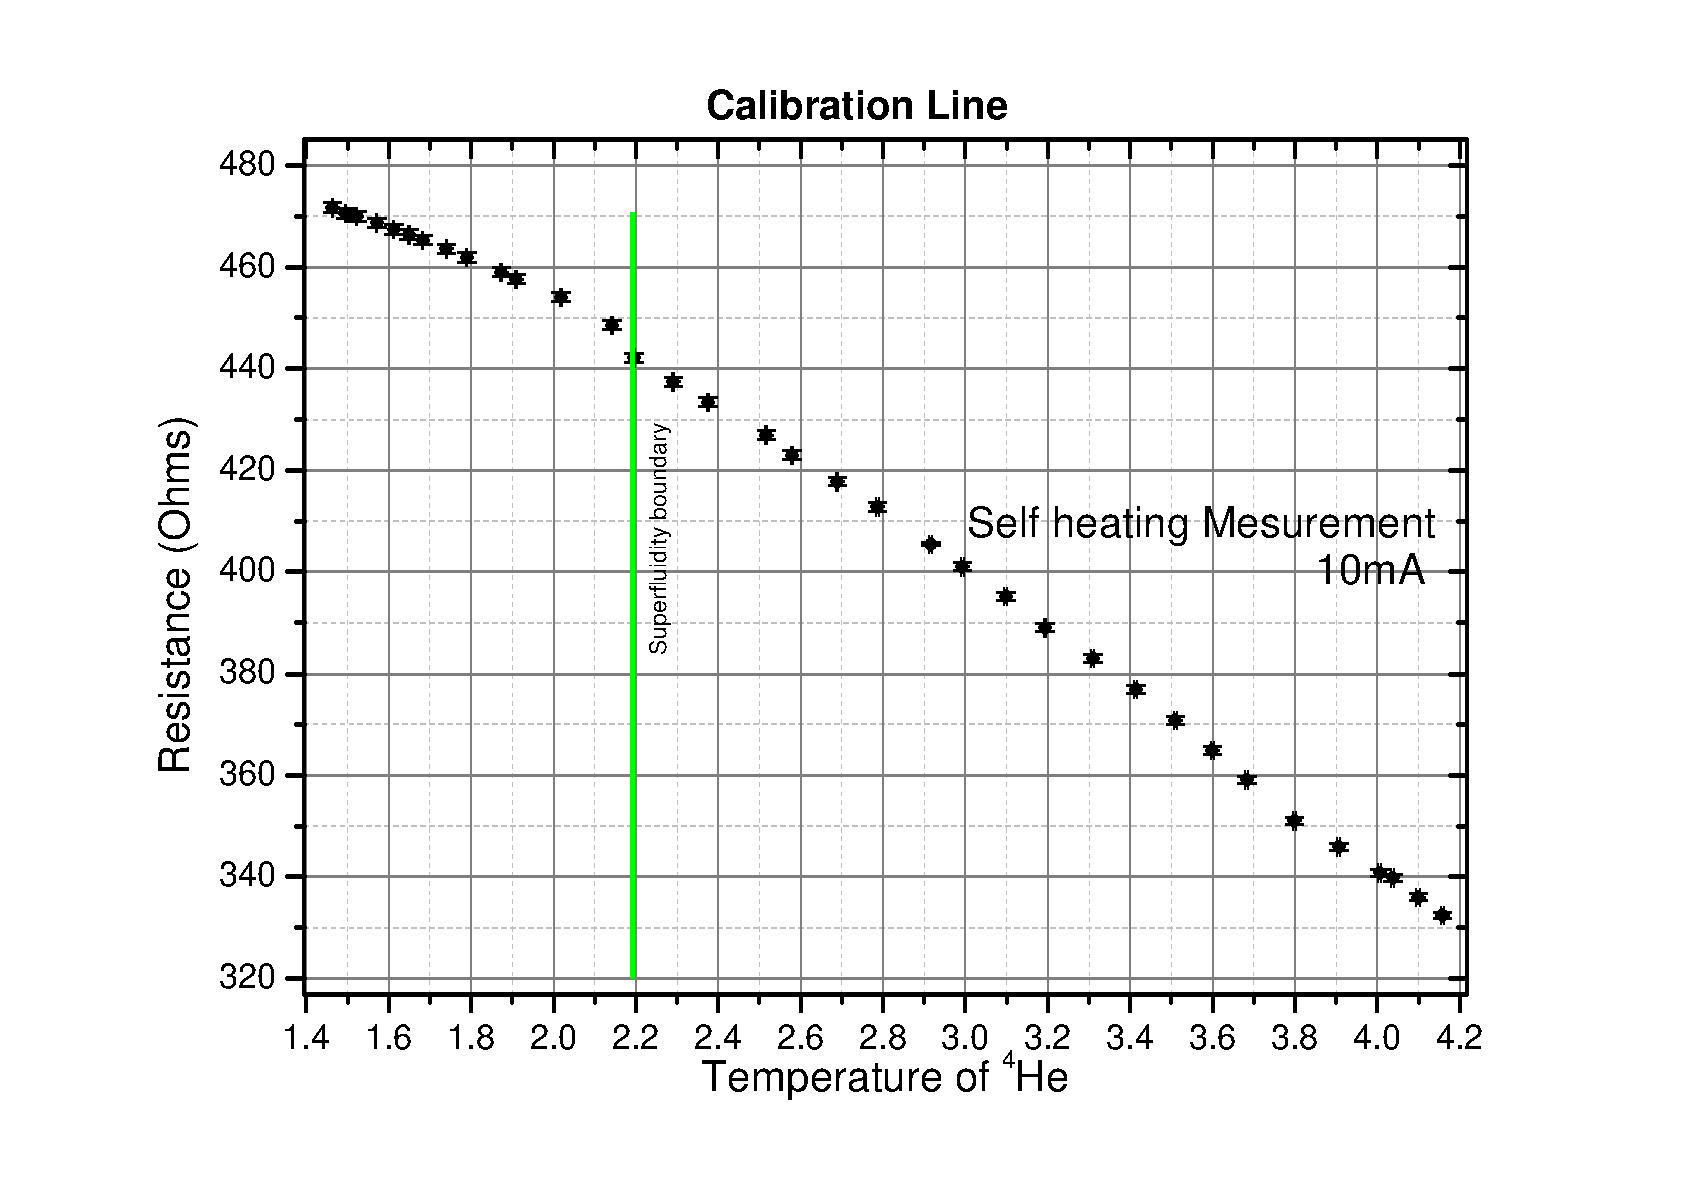
\includegraphics[width = 0.8\textwidth]{pics/selfheatingcali.pdf}
\caption{Full range of data taken with annotated superfluidity boundary.\label{fig:selfheatingcali}}
\end{figure*}

\begin{figure*}[htbp]
\centering
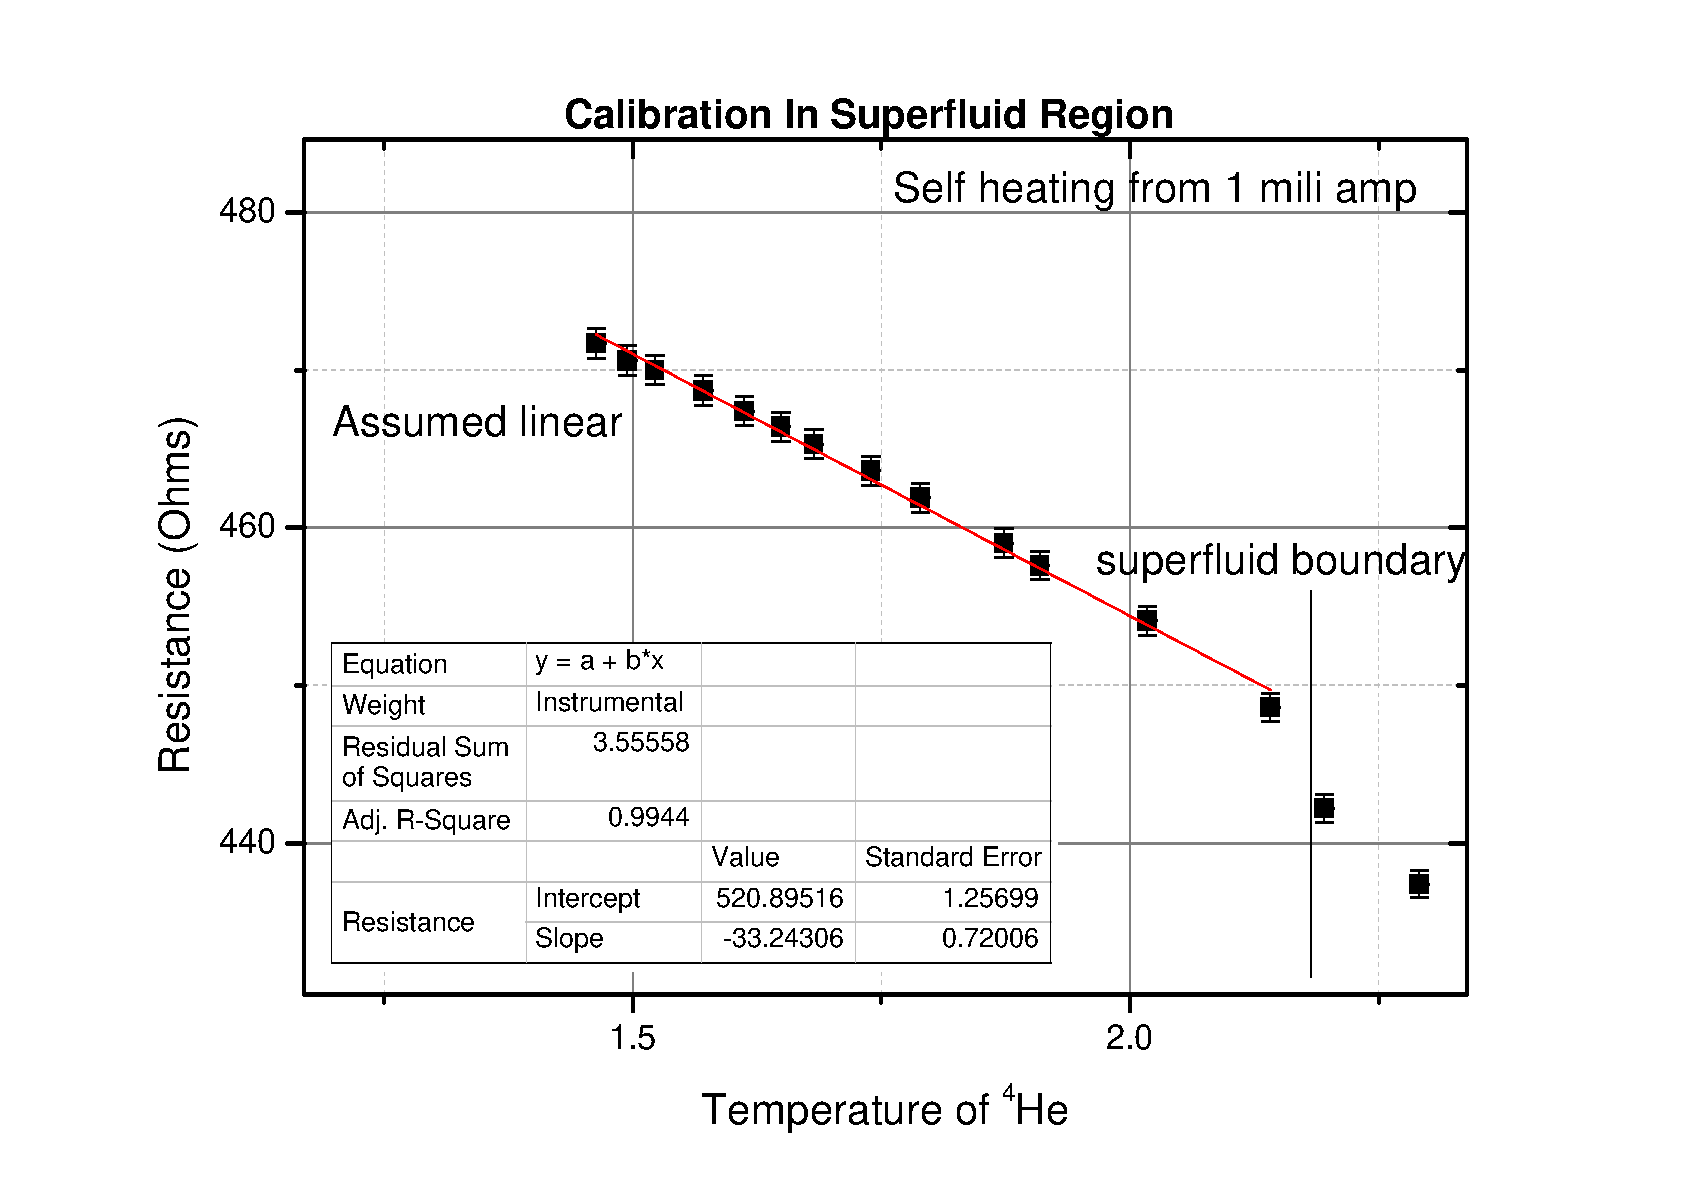
\includegraphics[width = 0.8\textwidth]{pics/calibrationline2.pdf}
\caption{Linear plot for calibration of resistance in the superfluid region\label{fig:calibrationline}}
\end{figure*}

For the superfluid the conversion from resistance $R$ in ohms to
temperature $T$ in kelvin is
\begin{equation}
\frac{R - (520.89\pm1.25)}{(-33.24\pm0.72)} = T
\end{equation}
For $R$ in the range $(448 \to 471)\Omega$.
The conversion add an uncertainty of 2.17\% but as it is constant conversion
formulae over the range $(1.4 \to 2.3)$K so trends will keep there shape. 

A linear relationship for R againt T is not expected
although over a short range of $\Delta T$ it can be useful.

When the self-heating of the resistor was discovered and the measurement scale changed
the additional data collected is plotted with the prior data, Figure \label{fig:calibrationselfheating}.
It shows that without the resistor heating itself the resistance is much higher and curved.


\begin{figure*}[htbp]
\centering
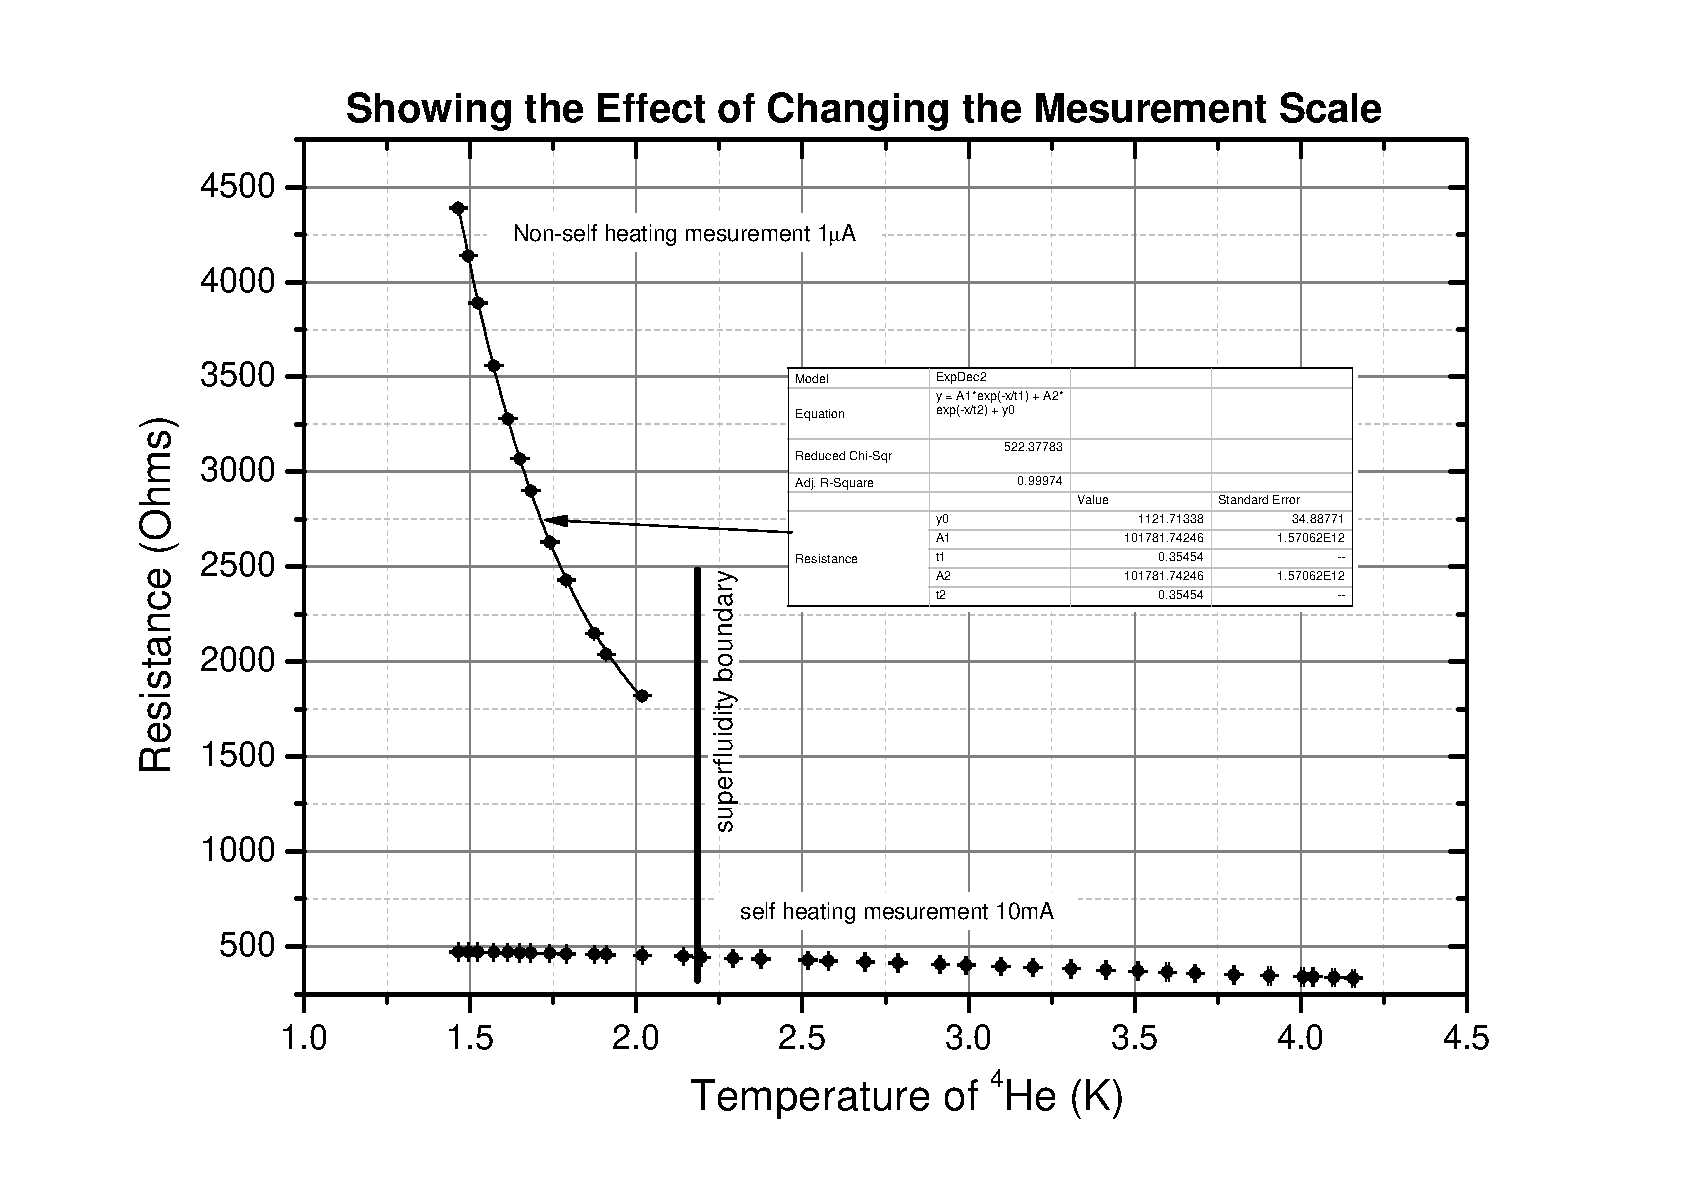
\includegraphics[width = 0.8\textwidth]{pics/calibrationselfheating2.pdf}
\caption{Plotting both sets of recoreded resistances showing the dramatic change
caused by self heating the resistor.\label{fig:calibrationselfheating}}
\end{figure*}

However the results are sill useful because the self heating effect is constant.
It is quite convenient to use the self-heating
calibration because it is liner rather than curved, it
is conceptually simpler, meaning conversions are simpler.
The non-self heating would yield better detail because of the range of resistances
and the better discrimination between measurements.

%also comment on the jump at t_lambda





